\label{chap:GANs}

Eine weitere Architektur, die zur Bildgenerierung verwendet werden kann, sind die sogenannten \emph{Generative Adversarial Networks} (\acsp{GAN}). \textbf{Auf Taxonomie eingehen} \textbf{Allgemeine Infos hinzufügen}.

Ein \ac{GAN} besteht aus zwei Komponenten. Dem sogenannten \emph{Generator} und dem \emph{Diskriminator} \emph{(engl.: Discriminator)}. Der Generator erzeugt aus einem zufälligen Eingangsvektor ein Bild. Der Diskriminator erhält ein Bild als Eingang und soll bewerten, ob das Bild echt oder künstlich generiert ist. Bei beiden Komponenten handelt es sich um \acp{KNN}. Das Ziel des Trainings ist, dass der Generator Bilder erzeugen kann, die der Diskriminator nicht von echten Trainingsbildern unterscheiden kann. Dabei wird der Generator besser in seiner Generierung, während der Diskriminator besser in seiner Unterscheidung wird. Je besser der Generator wird, desto besser muss der Diskriminator werden, um die Bilder unterscheiden zu können. Somit handelt es sich um ein direktes Gegenspiel zwischen Generator und Diskriminator. Das Zusammenspiel zwischen Generator und Diskriminator während des Trainings ist in Abbildung \ref{fig:gan} dargestellt. \cite{GANs}

\begin{figure}[H]
	\centering
	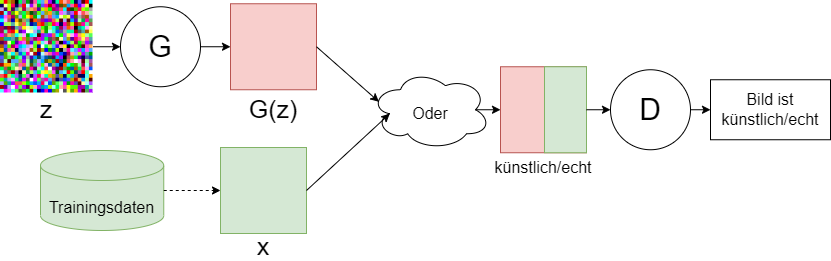
\includegraphics[width=0.8\textwidth]{../images/GANs/GAN.drawio.png}
	\caption{Zusammenspiel zwischen Generator und Discriminator}
	\label{fig:gan}
\end{figure}
Der Generator G erhält einen zufälligen Eingangsvektor $z$. Letzterer kann als ein weißes Rauschen beschrieben werden. Das generierte Bild ist das Resultat der Funktion $G(z)$ des Generators G. Anschließend wird dem Discriminator D entweder das generierte Bild $G(z)$ oder ein Bild $x$ aus den Trainingsdaten gezeigt. Der Ausganswert des Discriminators ist daraufhin die Einschätzung, ob das gezeigte Bild echt oder künstlich generiert ist. Ziel des Generators ist, dass die Verteilung der künstlichen Daten $p(G(z))$ möglichst ähnlich der Verteilung $p(x)$ ist. Der Discriminator soll die beiden Verteilungen möglichst gut voneinander unterscheiden können. Somit handelt es sich um ein direktes Gegenspiel zwischen Generator und Discriminator. Sie versuchen sich gegenseitig zu überlisten.

Im praktischen Einsatz wird nur der Generator verwendet. Der Discriminator wird ausschließlich dazu eingesetzt, mit $p(G(z))$ möglichst gut $p(x)$ zu approximieren, sodass die generierten Bilder im Optimalfall nicht von echten Trainingsdaten zu unterscheiden sind.
%Analog zu Kapitel \ref{chap:NoGANs}, ist die Aufgabe des Generators, Daten aus der Wahrscheinlichkeitsverteilung $p(x)$ der Trainingsdaten zu erzeugen. Der Eingangsvektor $z$ des Generators folgt einer Verteilung $p_z(z)$. Der Generator kann durch folgende Funktion beschrieben werden:

%\begin{equation}
%	G(z, \theta_{g})
%\end{equation}

%Der Generator erzeugt neue Bilder, während der Discriminator für jedes erzeugte Bild rät, ob es aus dem Trainingssatz stammt, oder ob es künstlich generiert ist. Nur der Discriminator hat dabei Zugriff auf den Trainingsdatensatz. Ihm werden klassischerweise abwechselnd Bilder aus dem Trainingssatz und erzeugte Bilder des Generators gezeigt. Die beiden Komponenten des \acp{GAN} agieren dabei stets gegeinander. Der Generator versucht den Discriminator in die Irre zu führen, dass seine generierten Bilder in Wahrheit aus dem Trainingssatz stammen würden, während der Discriminator versucht, möglichst gut zu erkennen, ob ein Bild echt ist oder nicht. Bei beiden Komponenten handelt es sich dabei um künstliche neuronale Netze \acused{KNN}(\acp{KNN}). \cite{visualApproach}

%\subsection{Spieltheorie}
%Aus spieltheoreticher Sicht kann das Gegenspiel von Generator und Discriminator auch als \emph{Nullsummenspiel} %betrachtet werden.

\subsection{Training}
Zu Beginn werden sowohl der Generator als auch der Discriminator mit zufälligen Parametern initialisiert. Dadurch ist zu erwarten, dass 


Der Generator erzeugt Bilder, die denen des Trainingssatzes nicht änhlich sind, während der Discriminator noch nicht weiß, was die Bilder des Trainingssatzes einzigartig macht. Durch das Training verbessern sich beide Komponenten in ihren Aufgaben. Sie trainieren sich gegenseitig, da sie beide versuchen, das Spiel zu gewinnen.

Das finale Optimum ist, dass der Discriminator so gut in der Unterscheidung zwischen echten und künstlichen Daten wird, wie mit den vorhandenen Daten nur möglich, während der Generator trotzdem in der Lage sein soll, den Discriminator zu überlisten. \cite[S. 656]{visualApproach}

Während die Bildklassifizierung ein Minimierungsproblem ist, stellt die Bildgenerierung mittels \acp{GAN} ein Min-Max-Problem dar. Bei ersterem wird versucht, die Loss-Function zu minimieren, sodass die Predictions möglichst gut den Labels der Daten entsprechen. Bei \acp{GAN} besteht der Unterschied darin, dass einerseits der Generator die Loss-Function zu minimieren versucht, während andererseits der Discriminator sie zu maximieren versucht.

\begin{equation}
	\min_{G} \max_{D} V(D,G) = \mathbb{E}_{x}[\log(D(x))] + \mathbb{E}_{z}[\log(1-D(G(z)))]
\end{equation}

(Auf Emfindlichkeit von GANs für Hyperparameter eingehen)

\subsection{Architekturen}
Die bisher beschriebene Architektur von \acp{GAN} wird auch als \emph{Vanilla \ac{GAN}} bezeichnet. Dies entspricht dem, wie \acp{GAN} in Goodfellows Publikation definiert werden \cite{Goodfellow-GANs}. Forscher und Anwender haben seit dieser Veröffentlichung verschiedene Limitationen und Probleme bei Vanilla \acp{GAN} feststellen können. Insbesondere im Hinblick auf spezielle Einsatzgebiete. Ein hier häufig anzutreffender Begriff ist \emph{Modal Collaps}. Damit ist die Situation gemeint, dass der Generator bei beliebigem Input stets dasselbe Bild generiert. Er lernt, dass ein bestimmtes Bild den Discriminator überlisten kann und generiert es deshalb jedes Mal, egal welchen Input man ihm zuführt. Lösen lässt sich dieses Problem beispielsweise mit sogenannten \acp{CycleGAN}.

\paragraph{CycleGANs}
Ein \ac{CycleGAN} besteht aus zwei miteinander gekoppelten \acp{GAN}. Diese werden klassischerweise als $G$ und $F$ bezeichnet. Bei $G$ handelt es sich um ein Vanilla \ac{GAN}, so wie in diesem Kapitel bisher beschrieben. Erweitert wird das Netzwerk jedoch so, dass es den Output von $G$ an $F$ weitergibt. $F$ erhält somit das von $G$ künstlich generierte Bild als Input. Aufgabe von $F$ ist, daraus den ursprünglichen Input, der $G$ zugeführt wurde, zu reproduzieren. Somit soll das gesamte Netzwerk nicht nur aus einem Input einen gewissen Output generieren können, sondern soll auch von einem gegebenen Output zurück auf den Input schließen können. Dies lässt sich mathematisch so darstellen, dass $G$ und $F$ folgende Abbildungen implementieren:
\begin{equation}
	\mathbf{G}: X\mapsto Y \: \wedge \: \mathbf{F}: Y\mapsto X
\end{equation}
Das Modell $G$ erzeugt somit aus einem gegebenen $X$ ein $Y$, wohingegen $F$ aus dem $Y$ auf das $X$ schließen soll. Die Behebung des Modal Collaps findet dadurch statt, dass das Netzwerk den Output $\tilde{X}$ von $F$ überprüft und diesen mit dem tatsächlichen Input $X$ vergleicht. Es wird überprüft, wie ähnlich sich $\tilde{X}$ und $X$ sind. Liegt eine zu hohe Diskrepanz vor, kann das Netzwerk darauf schließen, dass $G$ Outputs erzeugt, die nicht in direkter Abhängigkeit zu $X$ stehen. 

Was deutlich wird, ist dass hierbei die Idee verworfen werden muss, $G$ ein weißes Rauschen als Input zuzuführen. \acp{CycleGAN} sind für spezielle Anwendungsgebiete gedacht, in denen ausgewählte, und somit nicht-zufällige Eingabebilder verwendet werden. Dazu zählen Gebiete wie \emph{Style Transfer} oder die Transformation von Bildern, respektive Bildelementen. Es wird sich im Verlauf der Arbeit zeigen, dass die Problemstellung dieser Studienarbeit ein solches Anwendungsgebiet darstellt.

Adversarial Loss:
\begin{equation}
	L_{GAN}(G, D_Y, X, Y) = \mathbb{E}_y[\log{D_Y(y)}] + \mathbb{E}_x[\log(1-D_Y(G(x)))]
\end{equation}
Cyclic Loss:
\begin{equation}
	L_{cyc}(G, F) = \mathbb{E}_x[\mathcal{L}_{1}(F(G(x))-x)] + \mathbb{E}_y[\mathcal{L}_{2}(G(F(y))-y)]
\end{equation}
Total loss:
\begin{equation}
	L(G, F, D_X, D_Y) = L_{GAN}(G, D_Y, X, Y) + L_{GAN}(F, D_X, Y, X) + \lambda L_{cyc}(G, F)
\end{equation}
\cite{cycleGAN}

\todo[inline]{Erwähnen, dass die Loss-Funktionen in Implementierungen häufig zu Werten für generatorXLoss generatorYLoss, dicsriminatorXLoss und discriminatorYLoss aufgeteilt werden, statt der hier gezeigten Aufteilung.}

\paragraph{Conditional GANs}

\cite{DeepLearningBook}
\cite{visualApproach}